%%%%%%%%%%%%%%%%%%%%%%%%%%%%%%%%%%%%%%%%%
% Journal Article
% LaTeX Template
% Version 2.0 (February 7, 2023)
%
% This template originates from:
% https://www.LaTeXTemplates.com
%
% Author:
% Vel (vel@latextemplates.com)
%
% License:
% CC BY-NC-SA 4.0 (https://creativecommons.org/licenses/by-nc-sa/4.0/)
%
% NOTE: The bibliography needs to be compiled using the biber engine.
%
%%%%%%%%%%%%%%%%%%%%%%%%%%%%%%%%%%%%%%%%%

%----------------------------------------------------------------------------------------
%	PACKAGES AND OTHER DOCUMENT CONFIGURATIONS
%----------------------------------------------------------------------------------------
\documentclass[
	a4paper, % Paper size, use either a4paper or letterpaper
	10pt, % Default font size, can also use 11pt or 12pt, although this is not recommended
	unnumberedsections, % Comment to enable section numbering
	twoside, % Two side traditional mode where headers and footers change between odd and even pages, comment this option to make them fixed
]{LTJournalArticle}

\addbibresource{sample.bib} % BibLaTeX bibliography file

\runninghead{Shortened Running Article Title} % A shortened article title to appear in the running head, leave this command empty for no running head

\footertext{\textit{Journal of Biological Sampling} (2024) 12:533-684} % Text to appear in the footer, leave this command empty for no footer text

\setcounter{page}{1} % The page number of the first page, set this to a higher number if the article is to be part of an issue or larger work
\usepackage{times}
\usepackage{kotex}
%----------------------------------------------------------------------------------------
%	TITLE SECTION
%----------------------------------------------------------------------------------------

\title{Machine Learning-based Distributed Processing \\ for BrisT1D Blood Glucose Prediction} % Article title, use manual lines breaks (\\) to beautify the layout

% Authors are listed in a comma-separated list with superscript numbers indicating affiliations
% \thanks{} is used for any text that should be placed in a footnote on the first page, such as the corresponding author's email, journal acceptance dates, a copyright/license notice, keywords, etc
\author{%
	Chaewon Kim\textsuperscript{1}}

% Affiliations are output in the \date{} command
\date{\footnotesize\textsuperscript{\textbf{1}}Department of Intelligent Electronics and Computer Engineering, Chonnam National University}

% Full-width abstract
\renewcommand{\maketitlehookd}{%
	\begin{abstract}
		\noindent Predicting blood glucose levels is crucial in managing Type 1 diabetes. Traditional methods of prediction have limitations in terms of resource consumption, especially when dealing with large numbers of patients or extensive longitudinal data from long-term patient monitoring. In this study, we used machine learning techniques to predict blood glucose levels one hour ahead using distributed processing of participant data from the previous 6 hours. Among the machine learning techniques, we employed linear regression, decision tree, and gradient-boosted trees regression to predict blood glucose levels. The experimental results showed that linear regression achieved the highest accuracy. This study can contribute to helping patients' health by predicting blood glucose levels in Type 1 diabetes patients.
	\end{abstract}
}

%----------------------------------------------------------------------------------------

\begin{document}

\maketitle % Output the title section

%----------------------------------------------------------------------------------------
%	ARTICLE CONTENTS
%----------------------------------------------------------------------------------------

\section{Introduction}

Type 1 diabetes (T1D) is a chronic condition where the body fails to produce insulin, making it unable to regulate blood glucose levels. Without proper management, this condition can be life-threatening, requiring those affected to self-administer insulin injections. Blood glucose levels are influenced by numerous factors, including diet, physical activity, stress, illness, sleep, and alcohol consumption, making insulin dosage calculations complex. This constant need to anticipate and respond to factors affecting blood glucose levels places a significant burden on individuals with T1D.

Predicting future blood glucose levels is crucial for effective T1D management. While various algorithms have been developed for this purpose, their effectiveness is limited by the complexity of health data and numerous unmeasured variables. Furthermore, traditional prediction methods become resource-intensive when processing extensive longitudinal data from large patient populations. This study employs machine learning methods combined with distributed processing to predict future blood glucose levels using a newly collected dataset.



%------------------------------------------------

\section{Materials \& Methods}


The overview of study is in Figure \ref{fig:dataprocessing}.

\begin{figure}
	\centering
	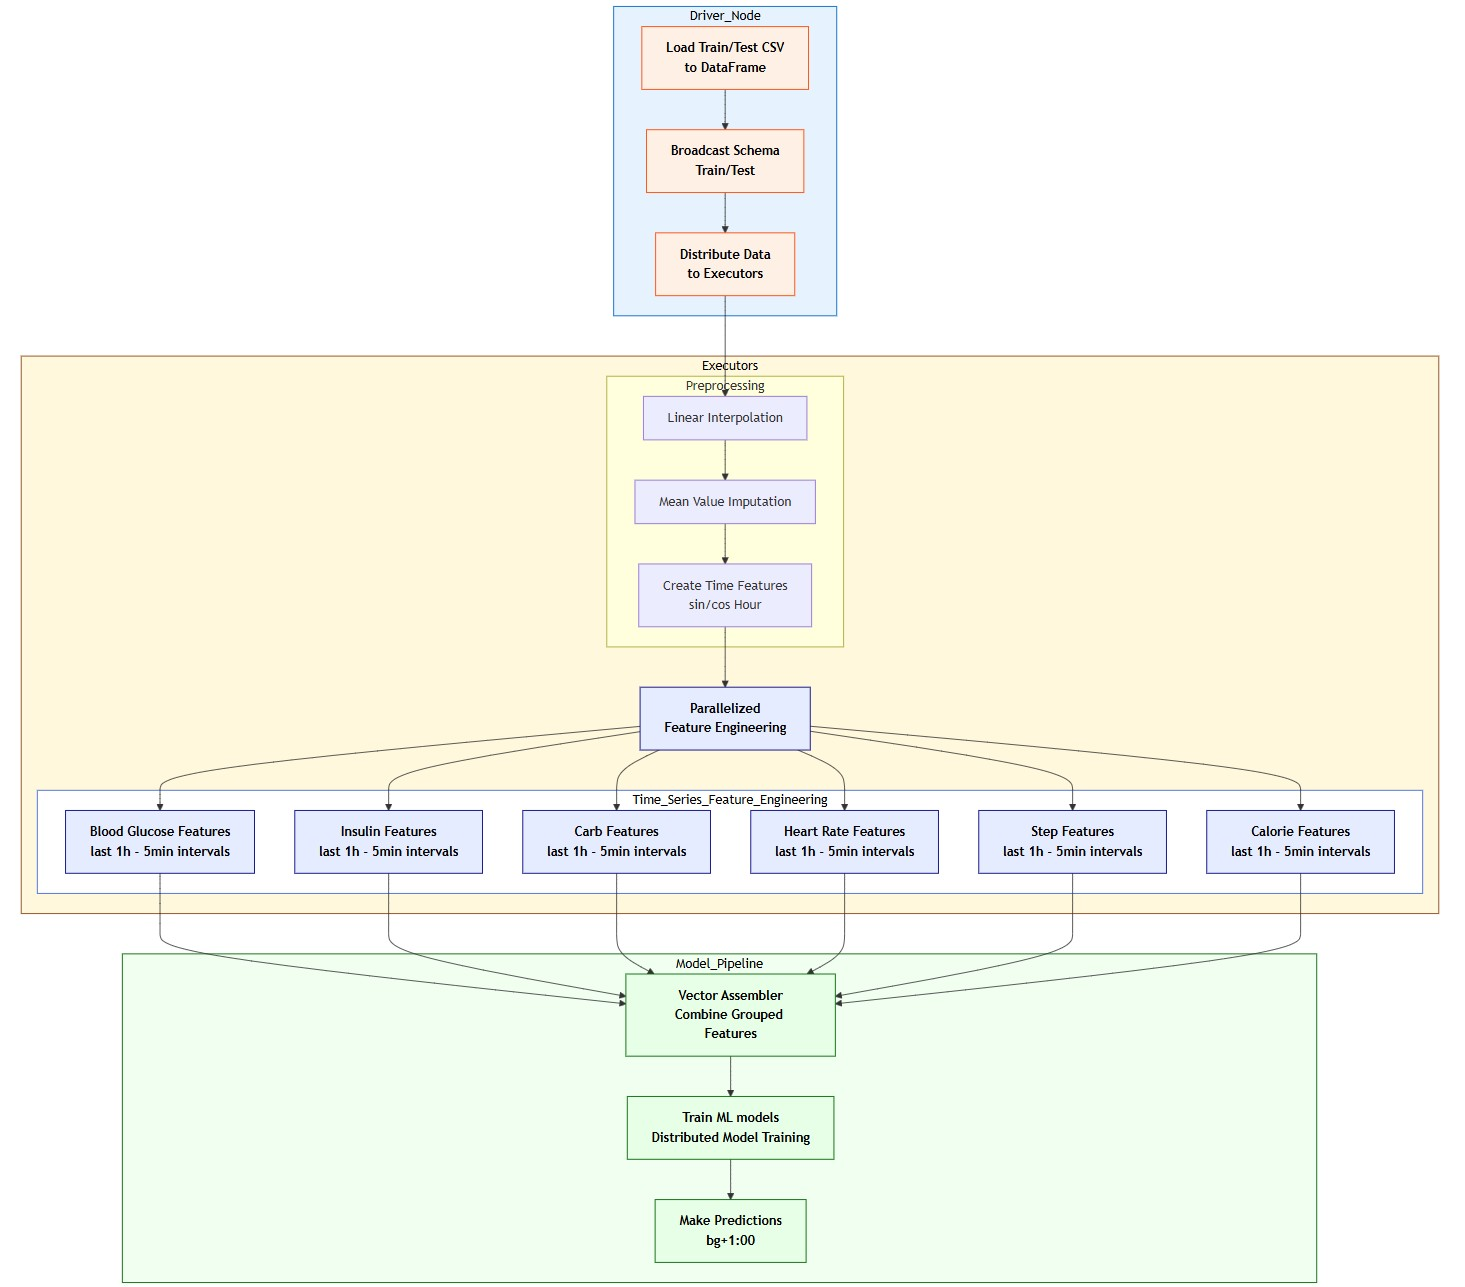
\includegraphics[width=1\linewidth]{./Figures/overview.jpg}
	\caption{Data processing pipeline.}
	\label{fig:dataprocessing}
\end{figure}

\subsection{Data sets}

The dataset is from a study that collected data from young adults in the United Kingdom with T1D diabetes, who used a continuous glucose monitor (CGM), an insulin pump and a smartwatch. These devices collected blood glucose readings, insulin dosage, carbohydrate intake, and activity data. The data collected was aggregated to five-minute intervals and formatted into samples. Each sample represents a point in time and includes the aggregated five-minute intervals from the previous six hours. The aim is to predict the blood glucose reading an hour into the future, for each of these samples.

The training set takes samples from the first three months of study data from nine of the participants and includes the future blood glucose value. These training samples appear in chronological order and overlap. The testing set takes samples from the remainder of the study period from fifteen of the participants (so unseen participants appear in the testing set). These testing samples do not overlap and are in a random order to avoid data leakage.

Complexities to be aware of:
\begin{itemize}
	\item This is medical data so there are missing values and noise in the data
	\item The participants did not all use the same device models (continuous glucose monitoring, insulin pump and smartwatch) so there may be differences in the collection method of the data
	\item Some participants in the test set do not appear in the training set
\end{itemize}


% \end{enumerate}

\subsection{Data Processing}

The training data consists of 177,024 rows and 508 columns, with a size of 296.59MB. Although the size is not particularly large, we applied distributed processing considering that the data volume could grow substantially in the future, as mentioned earlier. For this purpose, we utilized Apache Spark. The columns consist of hourly measurements of blood glucose, blood insulin concentration, carbohydrate intake, average heart rate, etc., with column names structured as "bg-X:XX".

To handle missing values, we performed linear interpolation on the time series data. For the date column representing time, we used sine and cosine transformations to generate periodic time features. This encoding allows us to capture the cyclical nature of daily time (e.g., 23:00 is close to 00:00). Additionally, we reduced the number of features by grouping columns that represent the same type of information.

\subsection{Modeling}

\subsubsection{Linear Regression}
Linear regression is a fundamental supervised learning algorithm that finds the best-fitting straight line through data points to predict outcomes. It became the first widely used regression method because of its simplicity and practicality - it creates models that have a linear relationship between variables, making them easier to understand and implement compared to non-linear models. The method works by learning from labeled data to create a linear function that can then be used to make predictions on new data points.


\subsubsection{Decision Trees}
Decision tree learning is a supervised machine learning method that creates a predictive model resembling a tree structure. It works by breaking down data through a series of decisions, where each branch represents a decision rule based on features, and each leaf represents an outcome. The method comes in two main varieties: classification trees for predicting discrete categories (like "yes/no" decisions), and regression trees for predicting continuous numerical values. This straightforward approach makes it particularly useful for both statistics and data mining tasks.


\subsubsection{Gradient-Boosted Trees Regression}
Gradient boosting is a powerful machine learning technique that creates strong predictions by combining multiple simple decision trees sequentially. Unlike traditional boosting methods, it uses pseudo-residuals in a functional space and optimizes any differentiable loss function. When specifically using decision trees as weak learners, the method is called gradient-boosted trees, which typically outperforms random forest by building the model in stages and allowing each new tree to correct errors from previous predictions.


\subsection{Evaluation}
The evaluation metric used in this study is the mean squared error (MSE). The MSE measures the average squared difference between the predicted values and the actual values. It is a common metric for regression problems, where lower values indicate better model performance. The MSE is calculated as follows:

\begin{equation}
	MSE = \frac{1}{n} \sum_{i=1}^{n} (y_i - \hat{y}_i)^2
\end{equation}

where $y_i$ is the actual value, $\hat{y}_i$ is the predicted value, and $n$ is the number of samples.

Features importance was also calculated for the decision tree and gradient-boosted trees models (Figures \ref{fig:DT_feature_importance}, \ref{fig:GBT_feature_importance}). Feature importance is a measure of how much each feature contributes to the model's predictions. It is calculated by the model during training and can help identify which features are most relevant for predicting blood glucose levels.


\begin{figure}[h!]
	\centering
	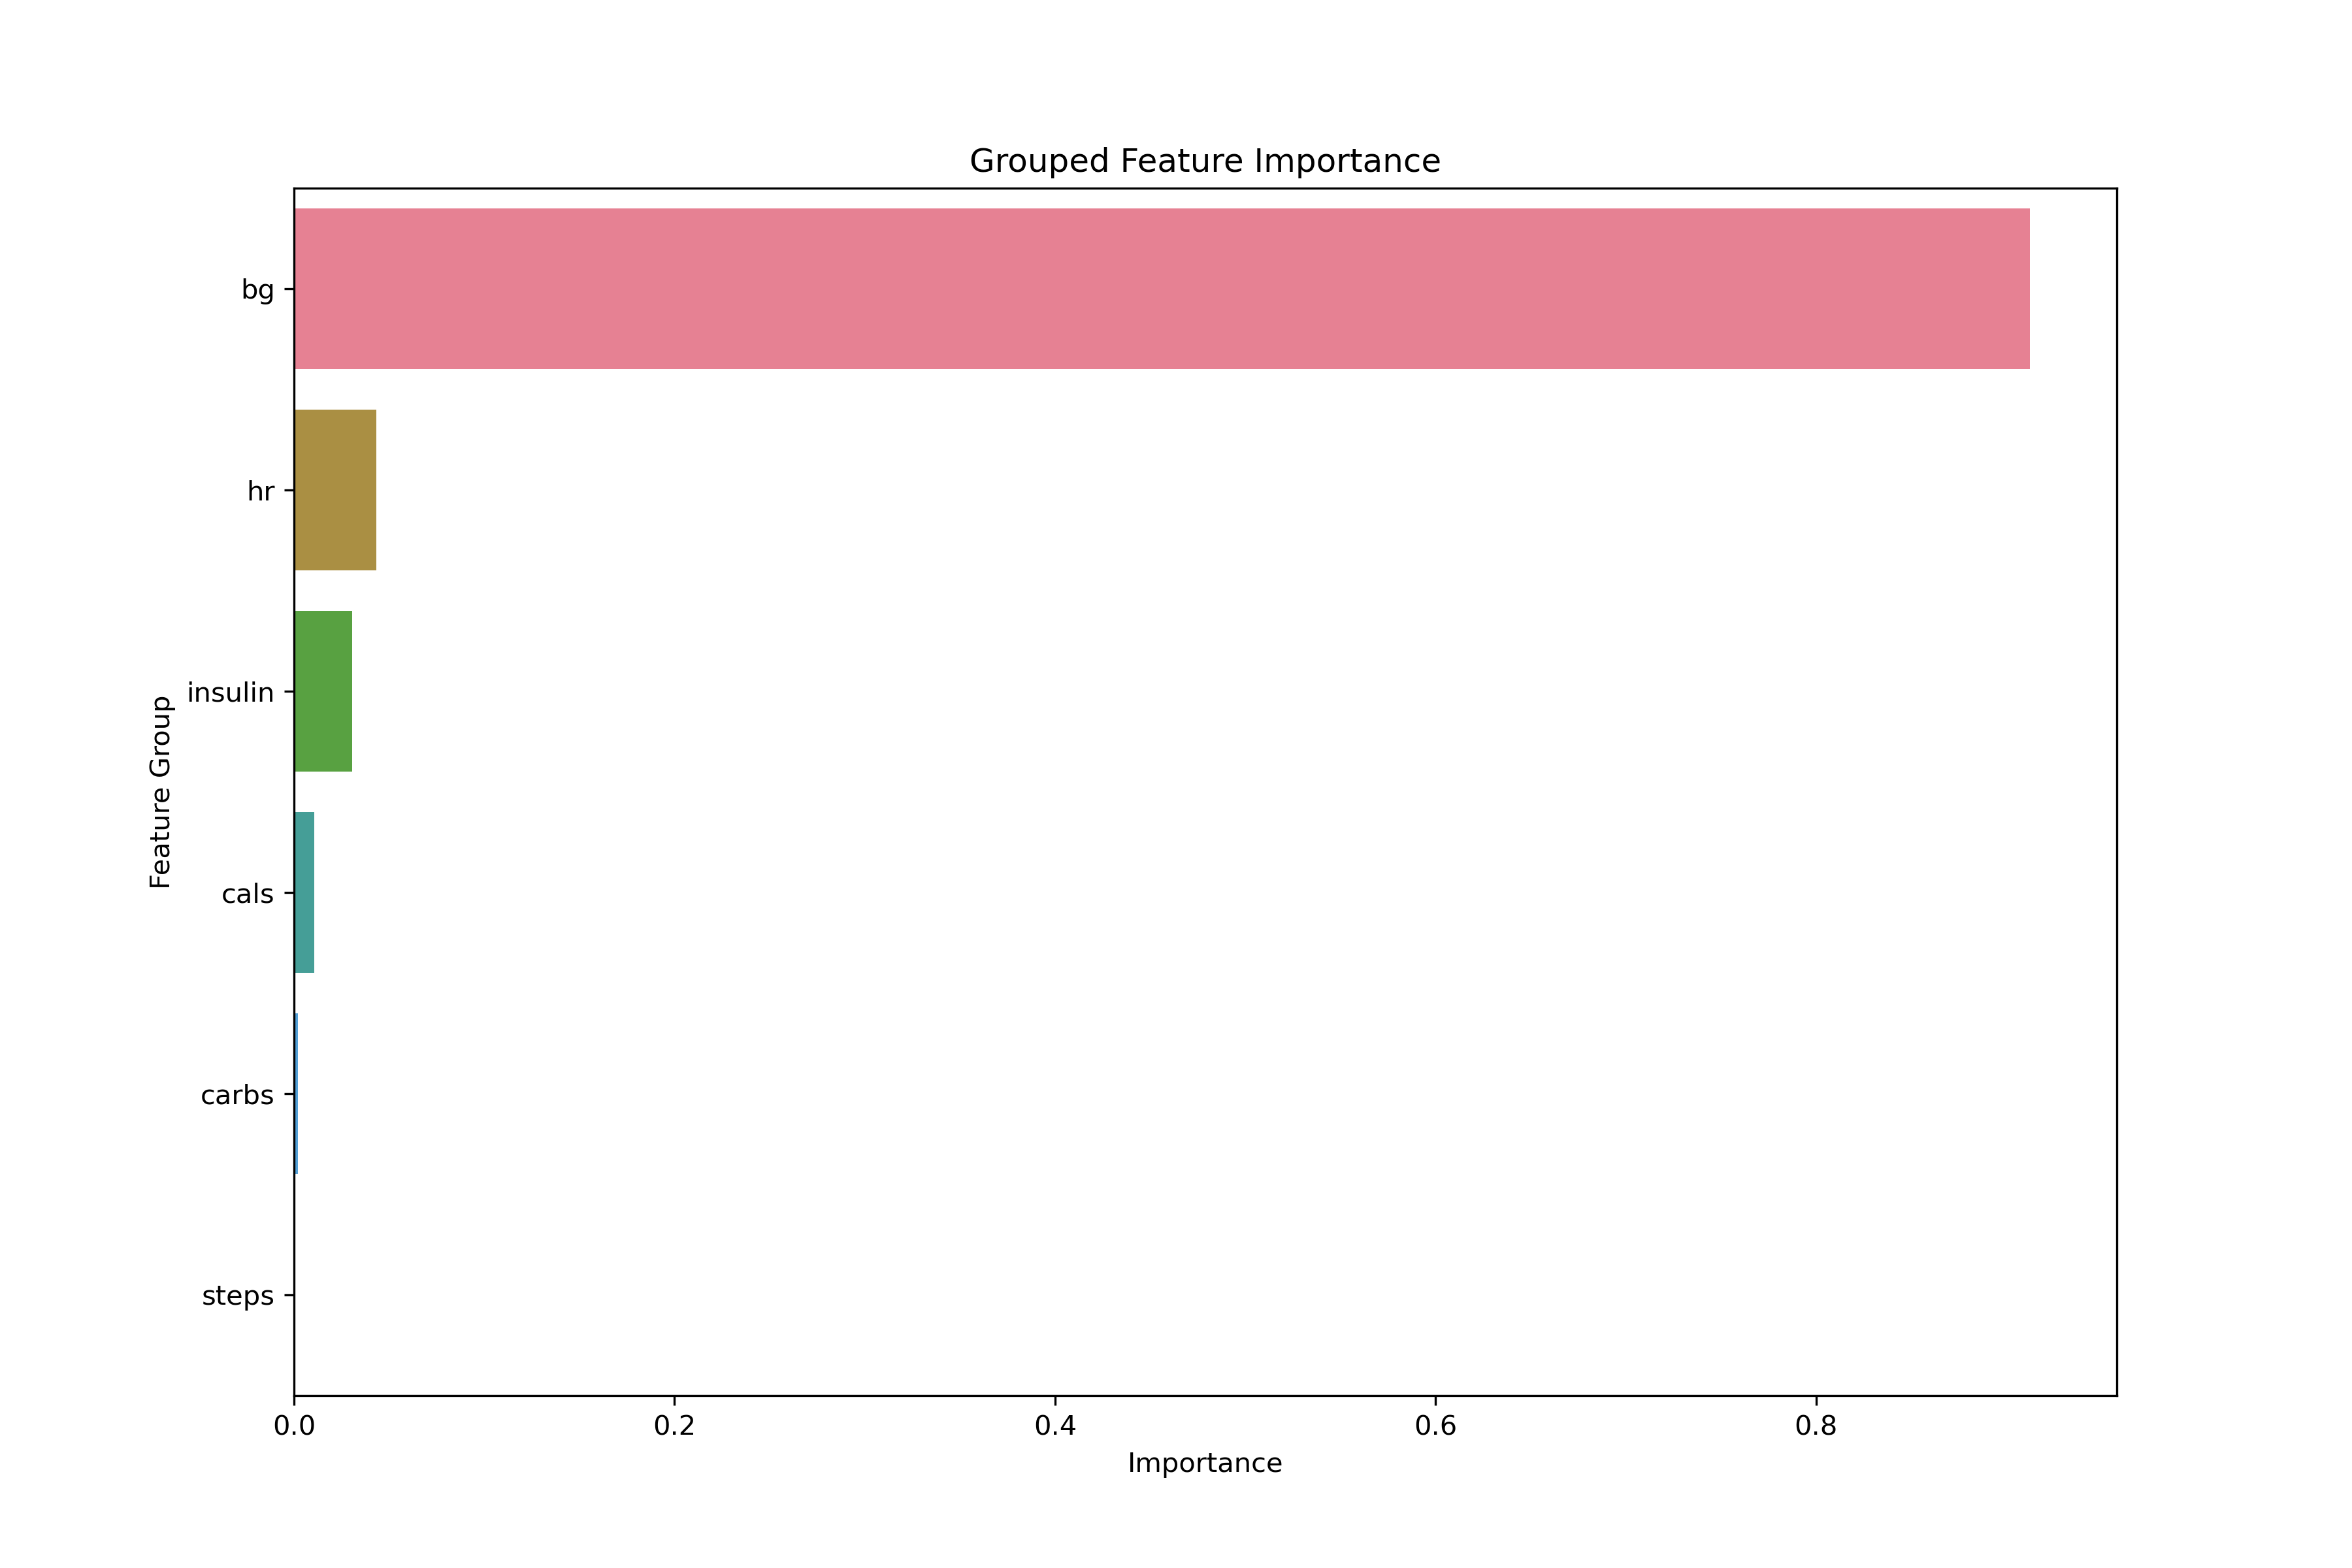
\includegraphics[width=1\linewidth]{../project_code/grouped_feature_importance_DT.png}
	\caption{Feature importance for the decision tree model.}
	\label{fig:DT_feature_importance}
\end{figure}

\begin{figure}[h!]
	\centering
	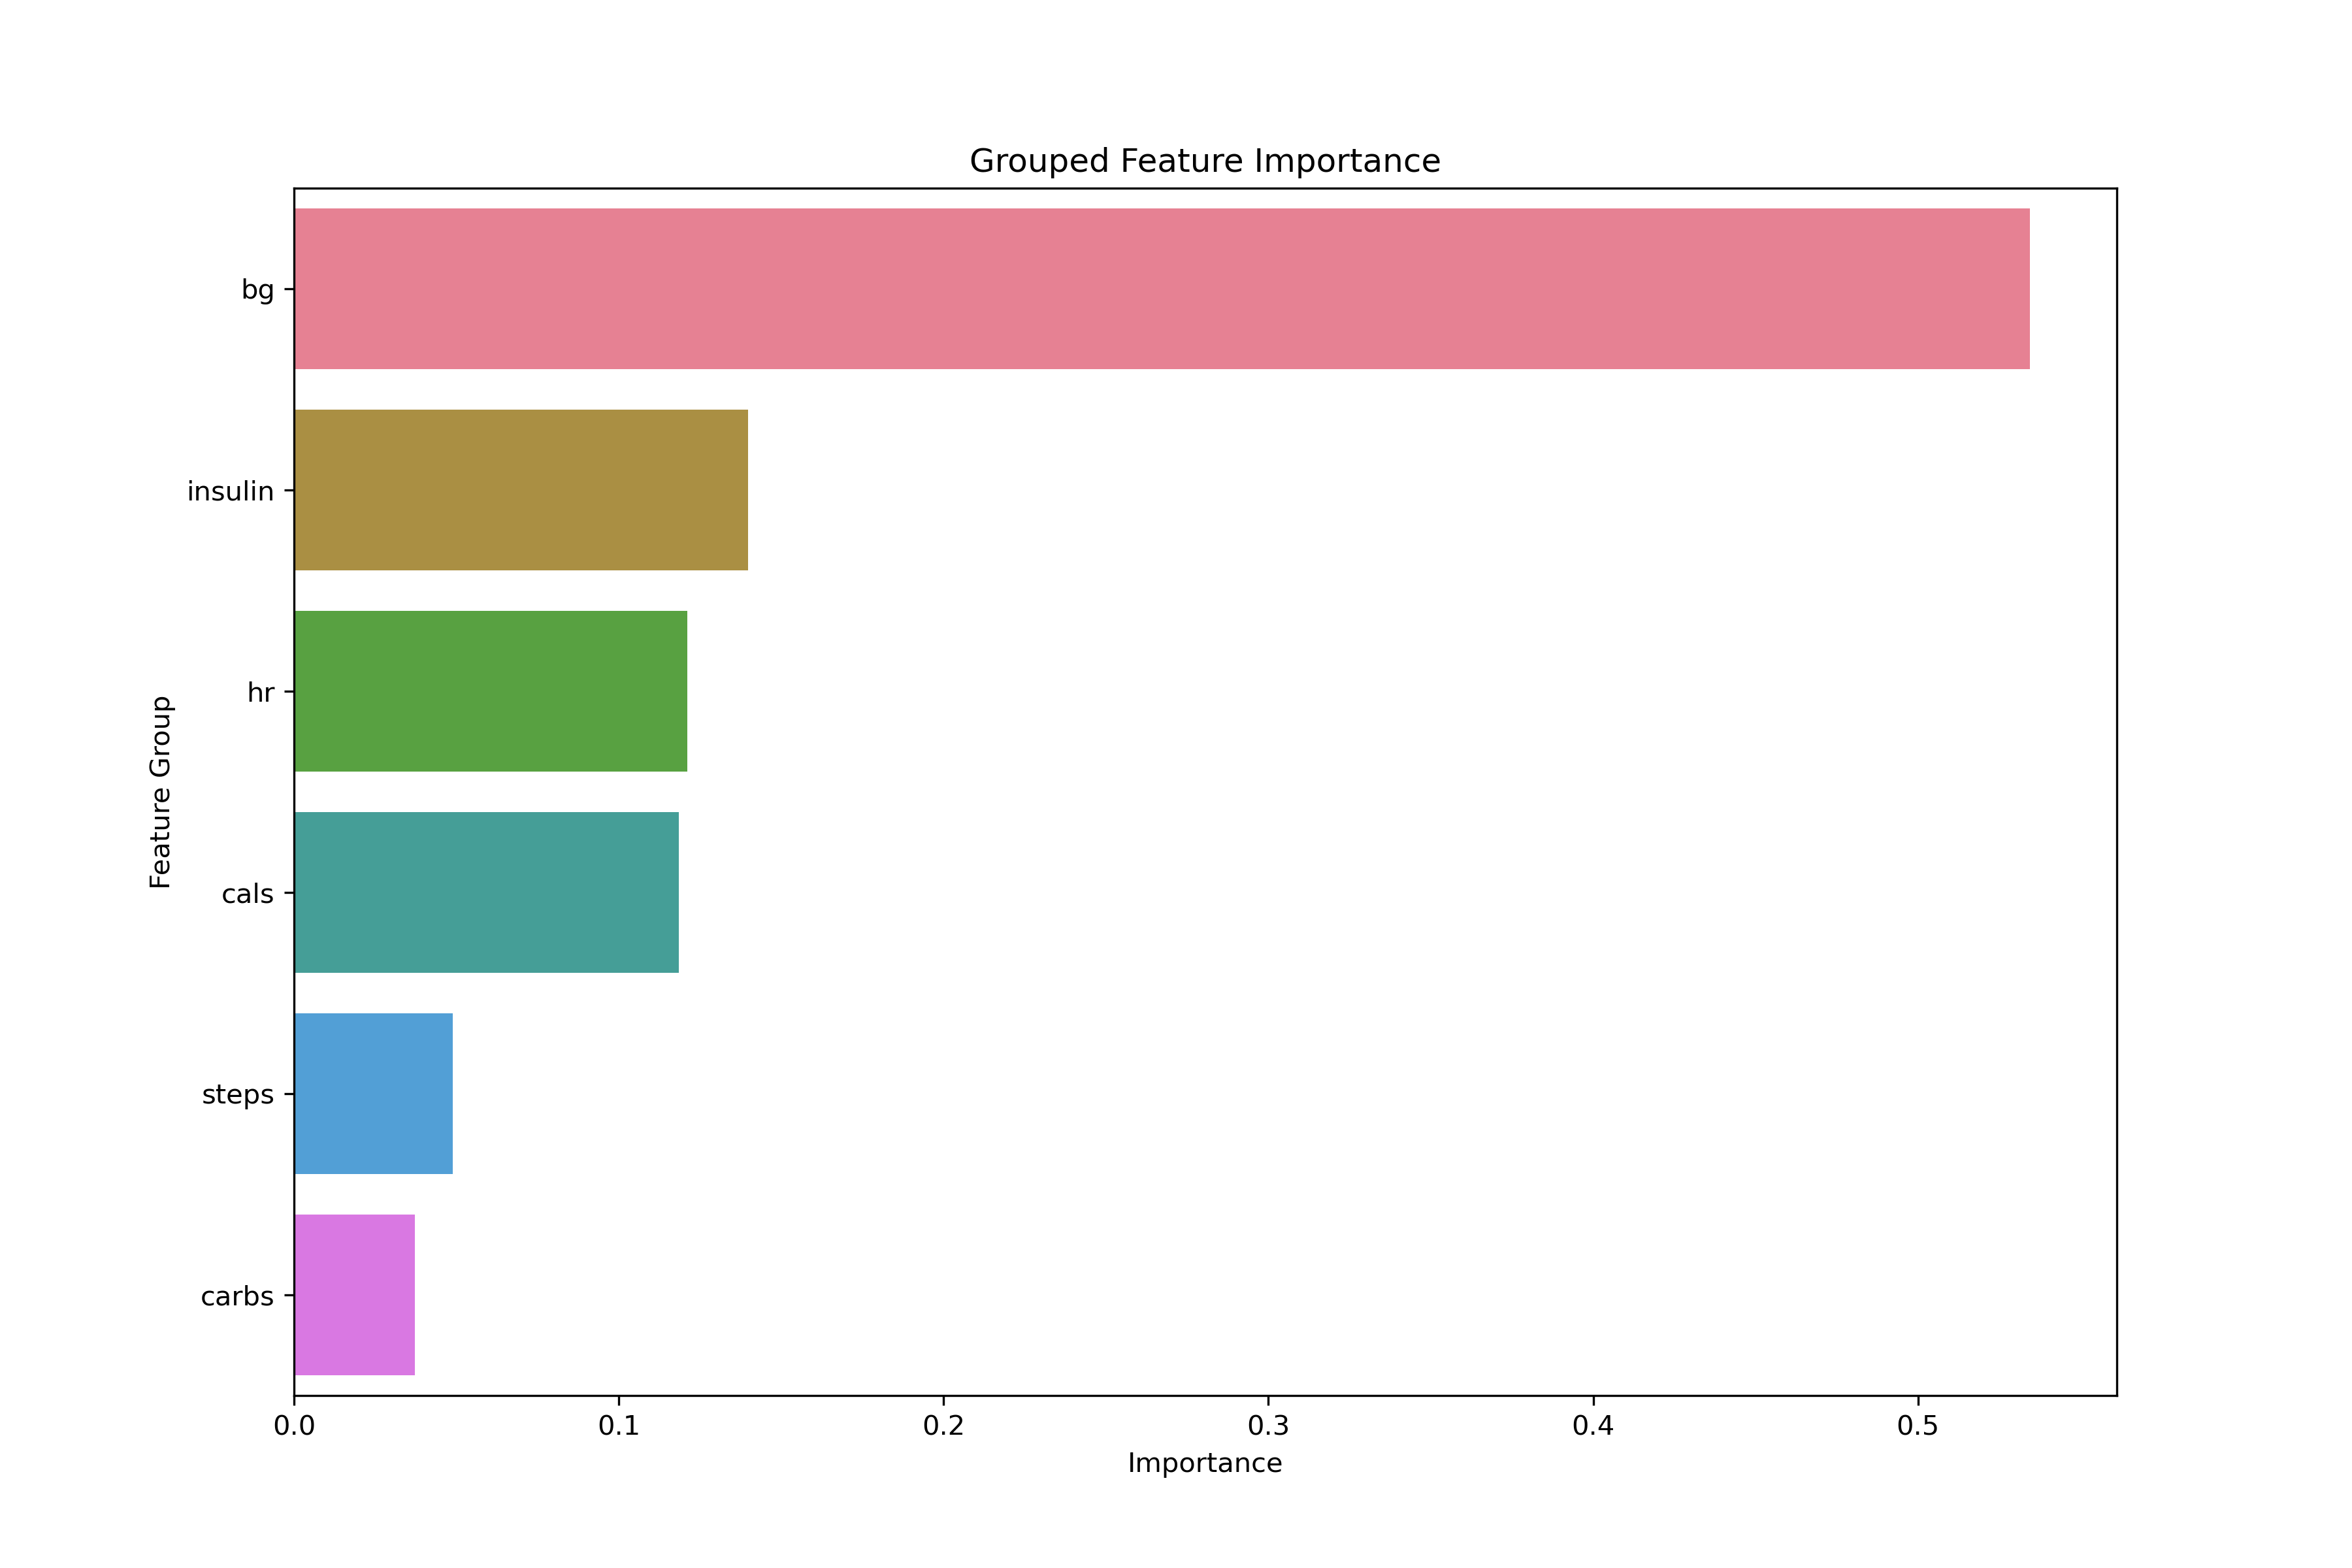
\includegraphics[width=1\linewidth]{../project_code/grouped_feature_importance_GBT.png}
	\caption{Feature importance for the gradient-boosted trees model.}
	\label{fig:GBT_feature_importance}
\end{figure}

%------------------------------------------------

\section{Results}

The results of models on the test set are shown in Table \ref{tab:distcounts}. The linear regression model achieved the lowest MSE of 2.64, followed by the gradient-boosted trees regression model with an MSE of 2.93, and the decision trees model with an MSE of 3.15. The linear regression model outperformed the other models, suggesting that it was able to predict blood glucose levels more accurately.

\begin{table}[h!]
	\caption{Model performance on the test set.}
	\centering
	\begin{tabular}{l r}
		\toprule
		Model & MSE \\
		\midrule
		Linear Regression & 2.64 \\
		Decision Trees & 3.15 \\
		Gradient-Boosted Trees Regression & 2.93 \\
		\bottomrule
	\end{tabular}
	\label{tab:distcounts}
\end{table}

%------------------------------------------------

\section{Discussion}

This study aimed to predict blood glucose levels in T1D patients using machine learning methods and distributed processing. The results show that linear regression outperformed the other models, with an MSE of 2.64. This suggests that the model was able to predict blood glucose levels, which could be beneficial for T1D patients in managing their condition.

There are several limitations to this study. The data used was from a small sample of participants, and the models may not generalize well to other populations. Additionally, the data was collected from different devices, which may introduce bias into the results. Future research could focus on collecting data from a larger and more diverse sample of participants to improve the generalizability of the models.

Overall, this study demonstrates the potential of machine learning methods to predict blood glucose levels in T1D patients. By accurately predicting blood glucose levels, these models could help patients better manage their condition and improve their quality of life.

The code is available on GitHub at \url{http://github.com/~~~~}


%----------------------------------------------------------------------------------------

\end{document}
